% GigaScience template
\documentclass[a4paper,num-refs]{oup-contemporary}

\journal{gigascience}


%%%% Packages %%%%
\usepackage{siunitx}
\usepackage{minted} % Used for JSON highlighting
\usepackage{algpseudocode} % Algorithmic environment
\usepackage{xspace}
\usepackage{booktabs}

%%%%%%

\usepackage{xcolor}
\usepackage{graphicx}
\usepackage{algorithm}
\usepackage{caption}
\usepackage{subcaption}
\usepackage{listings}
\usepackage{verbatim}
\usepackage{makecell}
\usepackage[flushleft]{threeparttable}

\usepackage{subcaption}
\usepackage{xspace}
\usepackage{stmaryrd} % for llbracket and rrbracket
\usepackage{amsmath}
\usepackage{ulem}
\usepackage{pifont}

\hypersetup{
colorlinks=true,% hyperlinks will be coloured
linkcolor=blue,% hyperlink text will be blue
linkbordercolor=blue,% hyperlink border will be blue
}
\makeatletter
\Hy@AtBeginDocument{%
  \def\@pdfborder{0 0 1}% Overrides border definition set with colorlinks=true
  \def\@pdfborderstyle{/S/U/W 1}% Overrides border style set with colorlinks=true
                                % Hyperlink border style will be underline of width 1pt
}
\makeatother

\DeclareMathOperator*{\argmin}{argmin}



%%%% Commands %%%%
% \newcommand{\todo}[1]{\color{red}\textbf{TODO:}#1\color{black}}
% \newcommand{\note}[2]{\color{blue}Note from \textsc{#1}: #2\color{black}}
\newcommand{\revision}[1]{\color{purple}\textbf{REVISION:}#1\color{black}}
\newcommand{\revised}[1]{\color{blue}#1\color{black}\xspace}
\newcommand{\reprozip}[0]{ReproZip\xspace}
\newcommand{\tristan}[1]{\color{orange}\textbf{From Tristan:}#1\color{black}}
\newcommand{\toolname}[0]{Spot\xspace}
\newcommand{\flirt}[0]{\texttt{flirt}\xspace}
\newcommand{\fnirt}[0]{\texttt{fnirt}\xspace}

\title{File-based localization of numerical perturbations in data analysis pipelines}
\begin{document}

\author[1]{Ali Salari}
\author[2,3]{Gregory Kiar}
\author[2]{Lindsay Lewis}
\author[2,3]{Alan C. Evans}
\author[1]{Tristan Glatard}

\affil[1]{Department of Computer Science and Software Engineering, Concordia University, Montreal, Canada}
\affil[2]{McGill University, Montreal, Canada}
\affil[3]{Montreal Neurological Institute, Montreal, Canada}

\maketitle

\begin{abstract}
Data analysis pipelines are known to be impacted by computational conditions, presumably due to the creation
and propagation of numerical errors. While this process could
play a major role in the current reproducibility crisis, the precise
causes of such instabilities and the path along which they propagate in
pipelines are unclear. We present \toolname, a tool to identify which
processes in a pipeline create numerical differences
when executed in different computational conditions. \toolname
leverages system-call interception through \reprozip to reconstruct and compare provenance
graphs without pipeline instrumentation. By applying \toolname to the
structural pre-processing pipelines of the Human Connectome
Project, we found that linear and non-linear registration are the cause of
most numerical instabilities in these pipelines, which confirms previous
findings.
\end{abstract}

% \begin{keywords}
% Computational reproducibility; Numerical instability; Neuroimaging.
% \end{keywords}


\section{Introduction}

% Reproducibility: crisis, numerical stability
% Containerization isn't the solution

\revised{Numerical perturbations resulting from variations in computational
environments} impact data analyses in various fields, but identifying the
origin of these perturbations in complex pipelines remains challenging.  In
some cases, small perturbations resulting from changes in operating system
versions~\cite{Glatard2015}, hardware~\cite{jezequel2015estimation}, or
parallelization parameters~\cite{diethelm2011limits}, result in
substantially different analysis outcomes, \revised{due to the propagation
and amplification of floating-point errors. While the existence of such
numerical errors is well known~\cite{stoer2013introduction}, their impact
on scientific computations has multiplied with the rise of the Big Data
era, due to the sustained growth of data sets, the increasing complexity of
analysis pipelines, and the diversification of computing infrastructures.}
To better understand and
correct these effects, efficient tools are
needed to assist pipeline developers
in the comparison of results obtained across different conditions.

In neuroimaging, our primary application field, data analyses often consist
of hundreds of computational processes -- often coming from multiple
toolboxes -- that are aggregated to perform a specific function. For
instance, the fMRIprep pipeline~\cite{esteban2019fmriprep} assembles software blocks
from FSL~\cite{jenkinson2012fsl}, AFNI~\cite{cox2012afni}, FreeSurfer~\cite{fischl2012freesurfer} and ANTs~\cite{avants2009advanced} to provide a state-of-the art
functional MRI processing tool with minimal user input. Another example are the pipelines of the Human
Connectome Project~\cite{glasser2013} that combine tools from FSL and FreeSurfer to pre-process
structural, functional and diffusion data from their
uniquely high-fidelity open dataset. In both cases, pipelines leverage toolboxes that are
widely trusted in the community, yet, at the same time substantial variations in results
have been observed in these toolboxes resulting from minor data
or infrastructure perturbations~\cite{Gronenschild2012, Glatard2015, Lewis2017-ll, kennedy2019everything}, suggesting that further investigation of their
numerical conditioning is required. For such complex pipelines, a
lightweight solution has to be found to perform such evaluations with
limited code instrumentation.

Numerical evaluations are traditionally performed using techniques such as
interval arithmetics~\cite{hickey2001interval} that require complete code re-writes and are
therefore barely applicable to complex pipelines. Recently, Monte-Carlo
Arithmetic~\cite{Parker1997-qq, Denis2016-wo} provided a practical way to
evaluate the uncertainty of numerical results without the need to rewrite
the application in a different paradigm. By perturbating floating-point
computations, it introduces a controllable amount of noise in the
pipelines, effectively sampling results from a random distribution. While
this technique is very appealing, it suffers from two main issues that make
it impractical at the scale of a complete pipeline. First, it requires that
all software components be recompiled for MCA instrumentation, which is not
always feasible. Second, it multiplies the execution time by a factor of 10
to 100, which is impractical when executions already take a few hours to
complete.

We present \toolname, a tool to identify the source of numerical differences in
complex pipelines without instrumentation. Using system-call interception
through the \reprozip tool~\cite{rampin2016reprozip}, \toolname traverses graphs of processes and
intermediary files to pinpoint the pipeline components that are unstable
across execution conditions. When differences start accumulating,
effectively masking any further instability, it restores clean data copies
through a set of wrapper scripts. Wrapper scripts are also used to restore
temporary data that might have been deleted during the execution, and to
disambiguate files that have been written by multiple processes. The remainder of this paper
presents the design of \toolname, and its
application to pre-processing pipelines of the HCP project.


% % Verificarlo and MCA, require recompilation
% Numerical instabilities originate in the limited \todo{precision} of floating-point representations.
% Traditionnaly, it has been evaluated through

% % -> File-based analysis of pipelines without instrumentation
% % Reprozip

% Reproducibility is a crucial element of the scientific works,
% as it enables researchers to evaluate authenticity and reliability
% of the findings~\cite{plesser2018reproducibility}.
% Reproducibility is defined as the ability to regenerate the same
% results as the original findings when the experiment is reanalyzed by
% the same analytic methods, software package, parameters, and
% data~\cite{peng2011reproducible}.
% In addition, numerical reproducibility is defined as the ability to
% regenerate bit for bit identical results from multiple
% runs~\cite{hill2017numerical}.
% We considered the numerical reproducibility in our experiments by comparing
% the binary content of the results using the checksum method.

% Recently, validation of the reproducibility has been widely investigated
% in the field of neuroimaging in which uses optimized
% processing methods with the purpose of functional and structural
% assessments of the human brain.
% According to the previous
% studies, the variety of computing infrastructures including workstation
% types, parallelization methods, operating systems, and analysis
% packages are known to influence the reproducibility of the analyses~\cite{Gronenschild2012,
% diethelm2012limits, Glatard2015, bowring2019exploring}.
% These irreproducibility issues are reported as the result of the
% creation, propagation, and amplification of small numerical
% differences.

% In particular, the effect of the operating systems on
% computational pipelines shows the creation of small numerical differences~\cite{Glatard2015, Scaria2017}.
% These differences mainly correspond to the mathematical functions implemented
% in different operating system libraries.
% For instance, changing the mathematical functions like \emph{expf()} and
% \emph{cosf()} which manipulate the precision of floating-point representations,
% between \emph{glibc} libraries in different operating systems can produce
% small numerical differences.
% Besides, a similar issue is expected for any operating system which is
% based on \emph{glibc}, the GNU C library.

% There are different approaches to improve the reproducibility of the analysis,
% including containerization techniques that encapsulate software/hardware dependencies,
% provenance capturing tools, and version control systems.
% However, a comprehensive solution requires to fix the numerical instabilities instead of
% masking the problem. For this purpose, bagging is one solution that has been used to
% stabilize motion estimation analysis in fMRI~\cite{Glatard2018hbm}.
% Bootstrap aggregation reduces the instabilities, but it needs expensive computations.
% As the second solution, a debugging tool can help to identify and
% fix the instabilities in the pipeline. Therefore, we introduce
% the numerical reproducibility measurement tool named \emph{Spot} to identify
% the processes in the pipeline that create numerical differences across different conditions.
% Furthermore, we can stabilize the identified processes in the next steps.



\section{Tool description}

\toolname identifies the components in a pipeline, at the resolution level of a system process, that produce different
results in different execution conditions. First, a directed
bipartite provenance graph is recorded for each pipeline execution, where nodes
represent application processes and files, and edges represent read and
write file accesses (Figure~\ref{fig:provenance-graph}). Second,
transient files, i.e., files that are either deleted during pipeline
execution or modified by multiple processes, are identified and
disambiguated, resulting in a provenance DAG (Directed Acyclic
Graph) in which file nodes have a single parent (in-degree of 1) (Figure~\ref{fig:provenance-dag}).
DAGs produced in different conditions are then compared, in
a step-by-step execution that prevents the propagation of differences in the pipeline (Figure~\ref{fig:labeled-dag}).
 The resulting labeled graph identifies the
non-reproducible processes in the pipeline.


\begin{figure*}
  \begin{subfigure}[t]{0.3\linewidth}
    \centering
    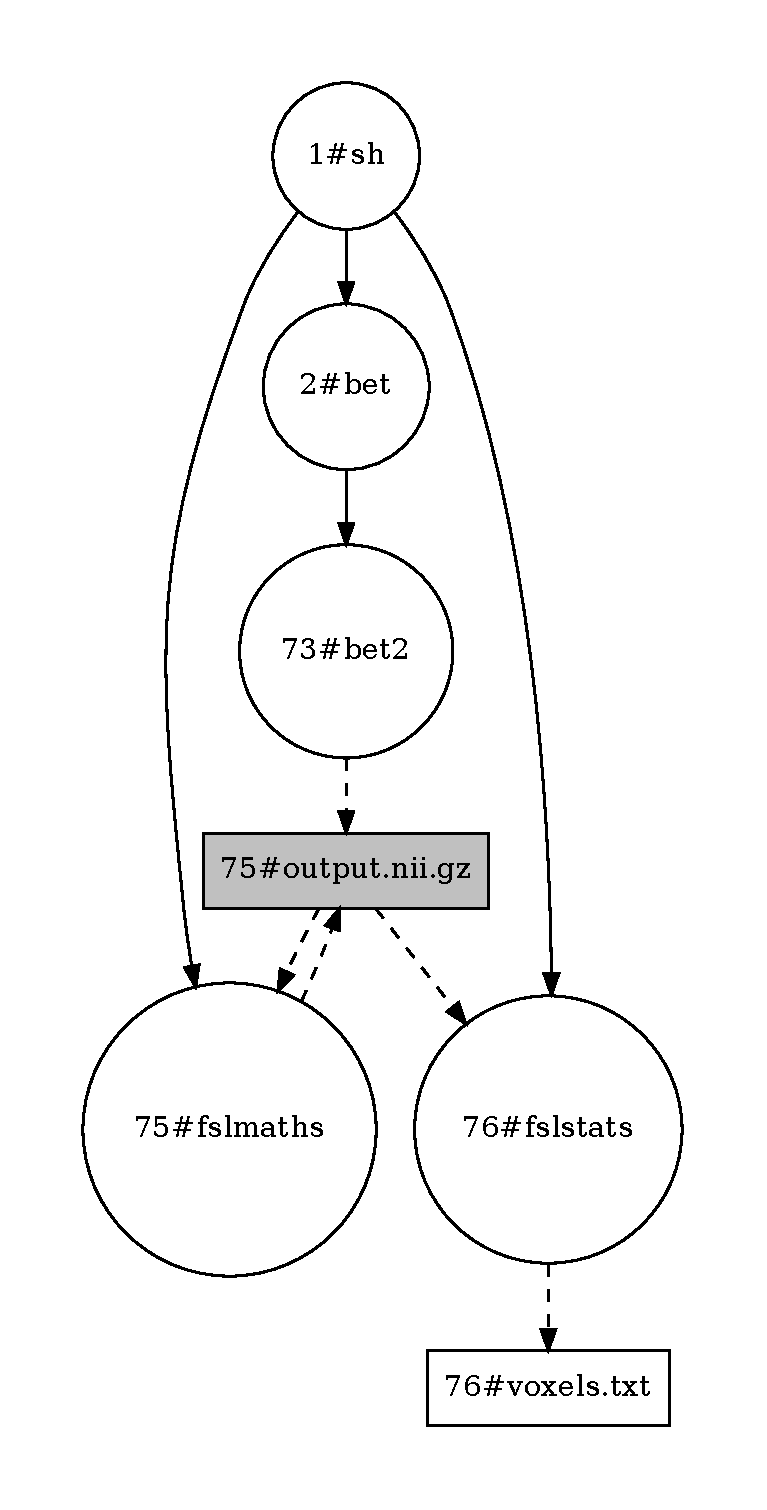
\includegraphics[width=.9\linewidth]{figures/p-graph.pdf}
    \caption{Raw provenance graph (\reprozip output), with transient files shown in gray boxes.}
    \label{fig:provenance-graph}
  \end{subfigure}
  \hfill
  \begin{subfigure}[t]{0.3\linewidth}
    \centering
    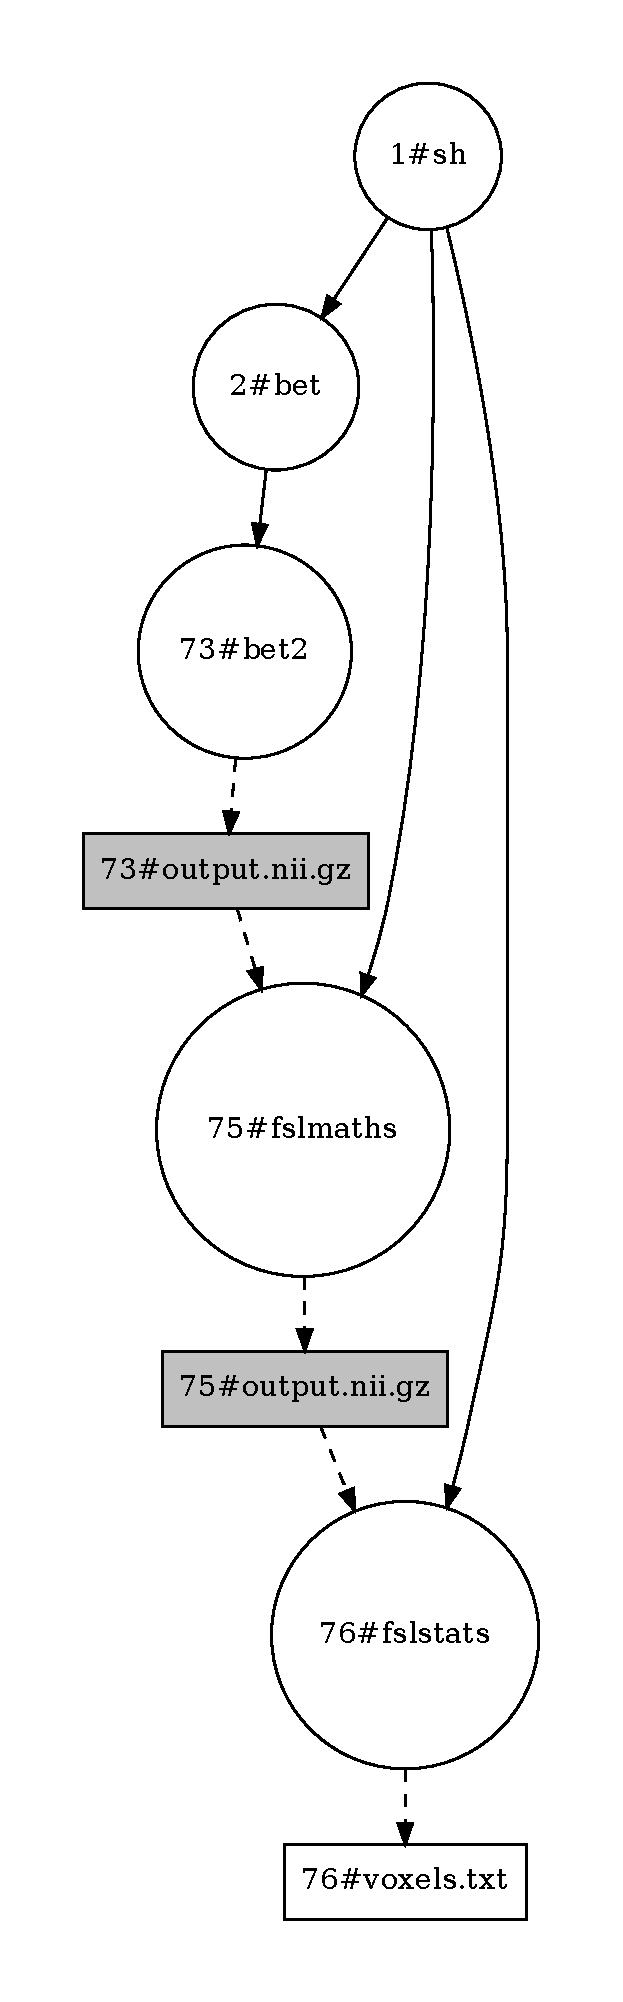
\includegraphics[width=.7\linewidth]{figures/p-graph-dag.pdf}
    \caption{Provenance DAG, with disambiguated transient files.}
    \label{fig:provenance-dag}
  \end{subfigure}
  \hfill
  \begin{subfigure}[t]{0.3\linewidth}
      \centering
      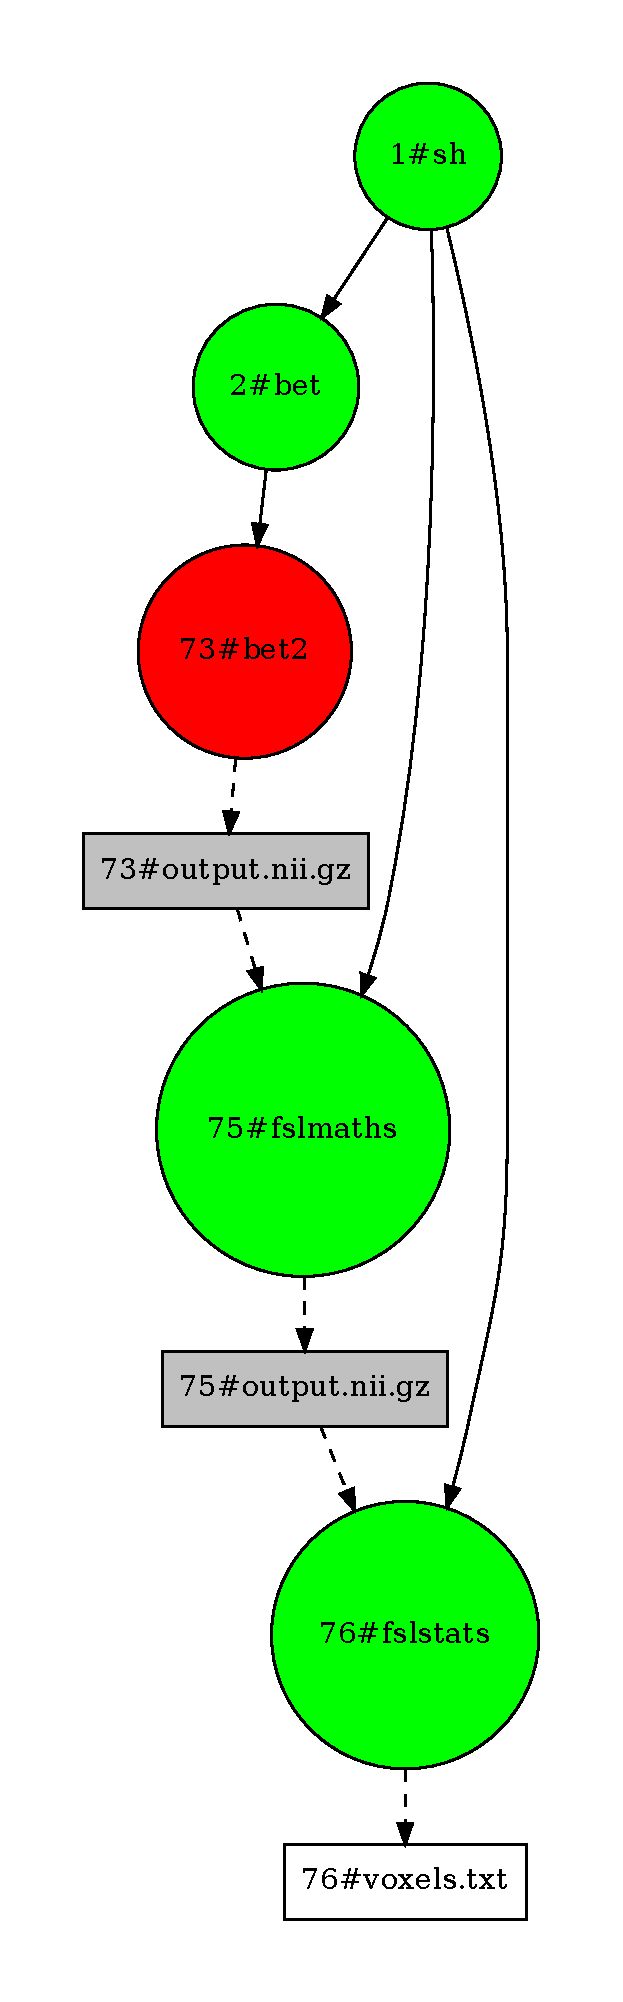
\includegraphics[width=.7\linewidth]{figures/p-graph-dag-labelled.pdf}
     \caption{Labeled DAG comparing 2 execution conditions, showing 1 non-reproducible process.}
     \label{fig:labeled-dag}
  \end{subfigure}
    % 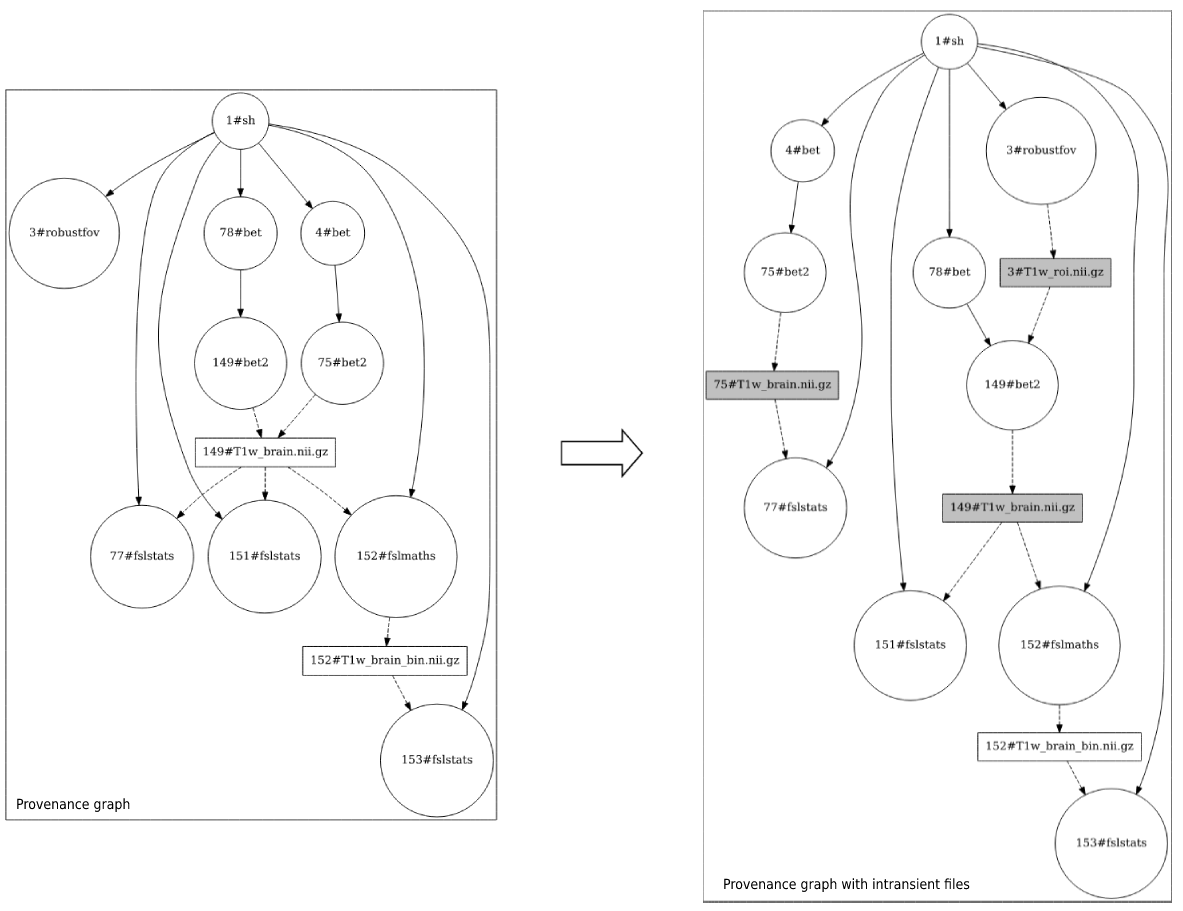
\includegraphics[width=.8\columnwidth]{figures/provenance-graphs}
    \caption{Provenance graphs created from the example pipeline in
    Listing~\ref{listing:sample-script}. Processes are represented with
    circles, files with rectangles, and read/write accesses with plain edges. For convenience, the process tree
    is also shown, with gray dashed edges. Processes forked by
    \texttt{bet} were captured by \reprozip while they did not appear in
    Listing~\ref{listing:sample-script}. Processed associated with
    executables located in \texttt{/usr/bin/} or \texttt{/bin/} are not shown.}
    \label{fig:spot-example}
  \end{figure*}

To ensure that a file can be unambiguously associated with the process that
created it, we assume that the pipeline can be transformed such that:
\begin{enumerate}
\item Processes don't run concurrently;
\item Each process sequentially reads, computes, and writes.
\end{enumerate}
In practice, pipeline processes may still run concurrently provided that
they don't write concurrently to the same files. A process may also
interleave file writes with computing, for instance when different file
blocks are processed sequentially. However, only a single version of the
file must eventually be made available to the other processes. In
particular, in case a process deletes a file that it had created itself,
this file must not be used by any other process. Finally, we also require that processes are
associated to a command line (executable and arguments), to facilitate
process instrumentation.

\begin{listing}
  \inputminted{bash}{"data/example/example.sh"}
  \caption{\revised{Example pipeline that computes the volume of the brain from a T1 image.}}
  \label{listing:sample-script}
\end{listing}

\subsection{Recording provenance graphs}

We use \reprozip~\cite{rampin2016reprozip}
to capture: (1) the set of processes created by the
pipeline, and
(2) the set of files read and written by each process, including
temporary files. \reprozip collects this information through the
\texttt{ptrace()} system call, with no required instrumentation of the pipeline.
Using the \reprozip trace, \toolname reconstructs a provenance graph by creating process and file
nodes and by adding directed edges corresponding
to file reads and writes (Figure~\ref{fig:provenance-graph}).
\revised{We assume that provenance graphs are identical for the \reprozip traces obtained from
the same subjects in different operating systems.}

Provenance graphs are often data-dependent, due to variations in input data that
may trigger differing branching or looping patterns across executions, for example.
%, which justifies the processing
% of multiple subjects. For instance, data acquisitions may be
% repeated a different number of times in each subject, for noise-reduction
% purposes.
Some of these differences can be neglected: for instance, when a data
decompression step is present at the beginning of the execution for some
subjects only. Other differences cannot: for instance, when entirely
different processing paths are used for different datasets. \toolname
includes helpers to identify different instances of provenance graphs,
such as supporting the clustering of process trees, where nodes are processes and
edges are \texttt{fork()} or \texttt{clone()} system calls, using the tree
edit distance~\cite{zhang1989simple} implemented in Python's \texttt{zss} package.

\subsection{Capturing transient files}

We capture temporary files by replacing every
process $P$ by a wrapper that first calls $P$ and then saves the produced
temporary files to a read-only directory. This process replacement is done by pre-pending
 to the \texttt{PATH} environment
variable a directory that contains a wrapper script named after the executable
called by $P$.

Files written by multiple processes are disambiguated using a similar technique. For a
 file $F$ written by the processes in \textbf{P} = \{$P_{1}$, \ldots,
 $P_{n}$\}, we first check that processes in \textbf{P} do not
 write concurrently to $F$, which would violate our assumptions. Then, we
 replace every process $P_{i}$ by a \texttt{PATH}-based wrapper that first
 calls $P_{i}$ and then saves $F$ to a read-only directory. In this way,
 successive versions of $F$ are preserved for comparison. We finally
 update the provenance graph accordingly, so that all files in the graph
 have an in-degree of 1 (Figure~\ref{fig:provenance-dag}). This operation also makes the provenance graph
 acyclic, since we assumed that a process could only release a single version of a file.

\subsection{Labeling processes}

After capturing transient files in the first condition (i.e. operating system, library version, etc.),
we re-run the pipeline
step by step in the second one to label processes. The output files
created by a process in both conditions are compared: if no differences are found, the process is marked as
reproducible; otherwise, the process is marked as non-reproducible, and the
output files produced in the first condition are copied to the second one, to ensure
that differences do not propagate further in the pipeline. Processes are
instrumented transparently through a modification of the \texttt{PATH}
variable similar to the one described previously. By default, differences
in output files are identified by comparing file checksums. Other
comparison functions can also be defined for specific file types, for
instance to ignore file headers or file sections containing timestamps.
\toolname finally creates a labeled
provenance graph highlighting non-reproducible processes.

Figure~\ref{fig:labeled-dag} illustrates a hypothetical incremental
labeling of the example in Listing~\ref{listing:sample-script}. Process
\texttt{bet2} is labeled as non-reproducible (red) as it produces files
with differences. To prevent the propagation of these differences, the
files produced by \texttt{bet2} in Condition 2 are replaced with the
files produced by \texttt{bet2} in Condition 1. Processes
\texttt{fslmaths} and \texttt{fslstats} are then executed and
labeled as reproducible (green) as they produce files without differences.

\revised{
The labeled graph can differ depending on the order of executions in which condition we capture transient files 
or execute the pipeline to pinpoint the propagation of differences. Therefore, we label processes in two orders 
of execution, and then aggregate findings so that label processes as non-reproducible (red) if it creates 
different results in either order of executions.}

\subsection{Implementation}
\revised{
\toolname is implemented in Python (>=3.5). In this work we used \toolname version 0.2 and the following version of
the Python package dependencies: NumPy v1.19.0~\cite{oliphant2006guide} and Pandas v1.0.5~\cite{mckinney2011pandas},
for data manipulations, SciPy v1.5.1~\cite{2020SciPy-NMeth} and Scikit-learn v.0.23.1~\cite{pedregosa2011scikit}
for the clustering of provenance graphs, Zss v1.2.0~\cite{zhang1989simple} for tree distances,
\reprozip v1.0.11 for the capture of provenance traces, Docker v17.05~\cite{merkel2014docker} for
the edition of container images, and Boutiques v0.5.25~\cite{glatard2018boutiques} for uniform pipeline executions.

Software users will mostly have to interact with the Boutiques and \reprozip packages.
Boutiques is a flexible description framework for containerized pipelines, required by
the pipelines analyzed in \toolname. It provides a JSON schema to describe inputs, outputs and their dependencies.
Examples, tutorials and usage documentation are available at \url{http://boutiques.github.io}. \reprozip intercepts
system calls to identify the files and processes involved in a pipeline execution.
Before using \toolname, users have to collect \reprozip traces of their pipeline executions.
Examples in the \toolname documentation include \reprozip provenance capture.
More documentation on \reprozip is available at \url{https://www.reprozip.org}.}

\section{Experiments}

We applied \toolname to the minimal
pre-processing pipelines released by the Human Connectome Project
(\href{https://www.humanconnectome.org}{HCP}), a leading initiative in
neuroimaging.

% In this experiment, we analyse the numerical reproducibility of computational pipelines
% and identify the origin of differences across the operating systems.
% Two types of differences can occur in the subjects due to the differences
% in the operating systems. One is between-OS differences caused by the
% operating system library updates and the other type, within-OS differences
% occur as a result of the pseudo-random processes used in the pipelines.

% In particular, Spot tool is tested on the neuroimaging applications which are
% predominantly using mathematical libraries. Therefore, we expect to find
% differences as a result of changing the mathematical functions between operating system libraries.

% This section describes datasets and pipelines used for the analyses, and the way of data processing.

\subsection{HCP pipelines and dataset}

% We used our tool to evaluate the reproducibility of the pipelines from the Human Connectome
% Project .
% The HCP initiative is an effort to acquire and analyse
% brain connectivity data from 1200 healthy adults.
% It enables the neuroscience
% research community to discover relationships between brain circuits and
% individual behaviors. This helps to understand a wide range of brain disorders.
% The HCP project provides database services (ConnectomeDB) for storing and
% sharing primary and processed data freely, and data analysis pipelines that
% are available under an open-source license.

The HCP developed a set of pre-processing pipelines to process structural,
functional, and diffusion MRI data acquired in the project. We focus on HCP
pre-processing pipelines for structural data, and particularly
on PreFreeSurfer and FreeSurfer.
A detailed description of the analyses done by these
pipelines is available in~\cite{glasser2013}.
In summary, the PreFreeSurfer pipeline consists of the following steps:
\begin{itemize}
\item Gradient Distortion Correction (DC),
\item Alignment and Anatomical Average (AAve), T1w(s), T2w(s),
\item Anterior/Posterior Commissure Alignment (ACPC-A),
\item Brain Extraction (BExt),
\item Bias Field Correction (BFC),
\item Atlas-Registration (AR).
\end{itemize}
And the FreeSurfer pipeline consists of the following:
\begin{itemize}
\item Image downsampling,
\item T1w image registration,
\item T1w image segmentation,
\item Surface placement,
\item Surface registration.
\end{itemize}

We randomly selected 20 unprocessed subjects from the HCP data release S500
available in \href{https://db.humanconnectome.org}{the ConnectomDB
repository} as a subset of the 1200 Subject Release \revised{(see Supplementary Table S1)}.
For each subject, available data consisted of 1 or 2 T1-weighted images and 1 or 2
T2-weighted images, with $256 \times 320 \times 320$ voxels of size $0.7
\times 0.7 \times 0.7$ mm. Acquisition protocols and parameters are
detailed in~\cite{van2013wu}.

% HCP data collected from different types of imaging techniques, including
% structural imaging (sMRI), functional imaging (fMRI), and diffusion imaging (dMRI).
% The structural images include T1-weighted (T1w) and T2-weighted (T2w) images, which
% help in the diagnosis of brain injury.
% The images are indexed with a suffix if several scans of the same modality were acquired.
% For example, some data may include two T1w images with low and high resolutions.
% The functional images, including task-based fMRI and resting-state scans,
% enable the measurement of functional activations within brain areas.
% Diffusion imaging is another kind of MRI technique, which measures
% the anatomical connectivity between regions.

\subsection{Data processing}

We built Docker images for the HCP pre-processing pipelines v3.19.0
(PreFreeSurfer and FreeSurfer) in CentOS 6.9 (Final) and CentOS 7.4 (Core), available on
\href{https://hub.docker.com/r/bigdatalabteam/hcp-prefreesurfer/}{DockerHub}.
Container images contain the HCP software dependencies, including FSL
(version 5.0.6), FreeSurfer (version 5.3.0-HCP, CentOS4 build), and
Connectome Workbench (version 1.0).

% \revision{Using the \reprozip trace obtained from CentOS7,
% we captured transient files in CentOS6 and labeled pipeline processes in CentOS7.}
We processed the 20 subjects with PreFreeSurfer and FreeSurfer, using the 2 CentOS versions.
\revised{First, PreFreeSurfer was utilized to analyze the unprocessed data, and then its results 
from CentOS6 were used as the input of FreeSurfer in both conditions. 
We also used the ReproZip trace file captured in CentOS6 for labeling the processes in both pipelines.}
Each subject was processed twice on the same operating
system to detect within-OS variability coming from pseudo-random
operations. We compared pipeline results using  FreeSurfer tools \texttt{mri\_diff},
\texttt{mris\_diff}, and \texttt{lta\_diff}, to ignore execution-specific information such as file path or
timestamps. To compare segmentations $X$ and $Y$, we used the Dice coefficient defined as follows:
\[DICE=\frac{2|X \cap Y|}{|X| + |Y|}\]

\revised{
The Dice coefficient~\cite{dice1945measures} is a commonly used metric to validate medical image segmentation.
Dice values range from 0 to 1, with 1 indicating a perfect overlap between two segmentation results and 0 indicates no overlap.
Alternatively, the Jaccard coefficient~\cite{jaccard1912distribution} could be used;
there is a direct correspondence between both metrics.}

% Finally, to cluster the subjects, the threshold value is set to zero in the clustering method.
% Also, we used the nearest neighbor algorithm to calculate the distance between clusters.

\section{Results}
\revised{
All experiments were run on a machine with a 3.4GHz Intel Core i7 processor using 8 cores and 32GB of RAM running
the CentOS7 operating system and Linux kernel version 3.10.
The processing time, output file size, number of file accesses and number of processes observed in PreFreeSurfer
and FreeSurfer are shown in~Table~\ref{table:pipeline-stats}.
The scripts and analyses used to create the figures in this section are available at
\url{https://github.com/big-data-lab-team/HCP-reproducibility-paper}.

\begin{table*}[ht]
  \centering
  \begin{threeparttable}
  \caption{Execution statistics of the pipelines per subject.}
  \label{table:pipeline-stats}
  \begin{tabular}{ccc|cc}
  \toprule
  \multicolumn{1}{c}{} & \multicolumn{2}{c}{PreFreeSurfer } &   \multicolumn{2}{c}{FreeSurfer } \\

                          & \makecell{Mean}  &  \makecell{Standard error}  & \makecell{Mean}   &  \makecell{Standard error}   \\ \midrule
  Processing time (mins)  &     106.67       &     2.68                    &     650.25        &     8.88     \\
  Output file size (GB)   &     2.8          &     0.10                    &     4.15          &     0.15     \\
  Number of file accesses &     94,089       &     2,645                   &     62,729        &     984     \\
  Number of processes     &     8731         &     198                     &     4031          &     47     \\
  \bottomrule
  \end{tabular}
  \end{threeparttable}
  \end{table*}
}
% All experiments were run on a machine with a 3.4GHz Intel Core i7 processor
% and 32GB memory under the CentOS7 operating system.
% The average processing time per subject was approximately 2~hours (with standard error X)
% for PreFreeSurfer and 8~hours (with standard error X) for FreeSurfer.
% The average output file size was 2.7~GB (with standard error Y) for PreFreeSurfer
% and 4.1~GB (with standard error Y) for FreeSurfer.
%\tristan{Ali, are these numbers per subject or for 20 subjects? it's an average of 20 subjects}
% For each subject, PreFreeSurfer accessed 83K files and created 7.7K processes, and FreeSurfer accessed 62K files and
% created 4K processes.

% \subsection{Subject clustering}

% To reduce the number of provenance graphs to be examined, we cluster
% process trees using agglomerative hierarchical clustering, as implemented
% in SciPy~\cite{oliphant2007scipy}. We use the tree edit
% distance~\cite{zhang1989simple} between process trees, as implemented in
% the zss Python package. This distance is defined as the minimum number of
% edit operations to transform one tree into the other. Three edit operations
% are considered: node label modification, node removal, and node insertion.
% Each operation has an associated cost of 1.
% //If threshold is 0, why do we even need the edit distance?//
\begin{table}[b]
  \centering
  \begin{threeparttable}
  \caption{Types of provenance graphs in PreFreeSurfer.}
  \label{table:data-clusters}
  \begin{tabular}{cc|cc}
  \toprule
  Type   &   \makecell{Number of \\ Subjects}   &  \makecell{Number of \\ T1w images}          & \makecell{Number of \\ T2w images}   \\ \midrule
  1      &               9                      &  2 & 2 \\
  2      &               8                      &  1 & 1 \\
  3      &               1                      &  1 & 2 \\
  4      &               2                      &  2 & 1\\
  \bottomrule
  \end{tabular}
  \end{threeparttable}
  \end{table}

\subsubsection{Within-OS differences}

We did not observe any within-OS difference in PreFreeSurfer. In
FreeSurfer, we identified 2 processes leading to within-OS differences due
to the use of pseudo-random numbers: image registration with
\texttt{mri\_segreg}, and cortical surface curvature estimations with
\texttt{mris\_curvature}. Fixing the random seed used in FreeSurfer removed
these differences.
% \note{Greg}{can you make some statement on the magnitude of these differences?} \tristan{Ali, that's for you.}
% \note{Ali}{
% \texttt{mris\_curvature} produces surfaces like lh.inflated.K and lh.inflated.H,
% I only can see differences using \texttt{mri\_diff} command that it shows:

%   Volumes differ in pixel data

%   maxdiff   0.18604827 at 130715 0 0 0

% for lh.inflated.H and

%   Volumes differ in pixel data

%   maxdiff   0.85469627 at 130682 0 0 0

% for lh.inflated.K

% If you know other ways to check magnitude of differences please let me know.
% \texttt{mri\_segreg} produces different sum files (ASCII file in which summary statistics are saved),
% but differences belong to meta-data like hostname, date, and SynthSeed. We should remove \texttt{mri\_segreg}
% because it doesn't create data differences.
% The outputs of both executables are in Consider:/data/asalari/ali-tests/paper\_images/
% }

\subsubsection{Between-OS differences in PreFreeSurfer}
%\subsubsection{PreFreeSurfer pipeline analysis}

We identified four types of subjects with different PreFreeSurfer
provenance graphs (Table~\ref{table:data-clusters}). Differences between
subject types came from different numbers of T1 and T2 images in the
raw data. We verified that
the provenance graphs were identical for all subjects of the same type, for
both versions of CentOS.

Figure~\ref{fig:pfs_heatmap} shows the frequency of non-reproducible pipeline processes
in PreFreeSurfer.
The processes identified as non-reproducible were observed in linear registration
with FSL \flirt (in ACPC-Alignment, Brain Extraction, Distortion Correction, and
Atlas Registration), in non-linear registration with FSL \fnirt (in Brain Extraction
and Atlas Registration), and in image warping with FSL \texttt{new\_invwarp} (in Brain Extraction
and Atlas Registration). Differences were also observed in image mean
computations with FSL \texttt{maths}  (in Anatomical Average).
Figure~\ref{fig:complete_pfs} shows a complete PreFreeSurfer labeled DAG, localizing
the observed differences in the entire pipeline, for a given subject.
\begin{figure*}
\centering
  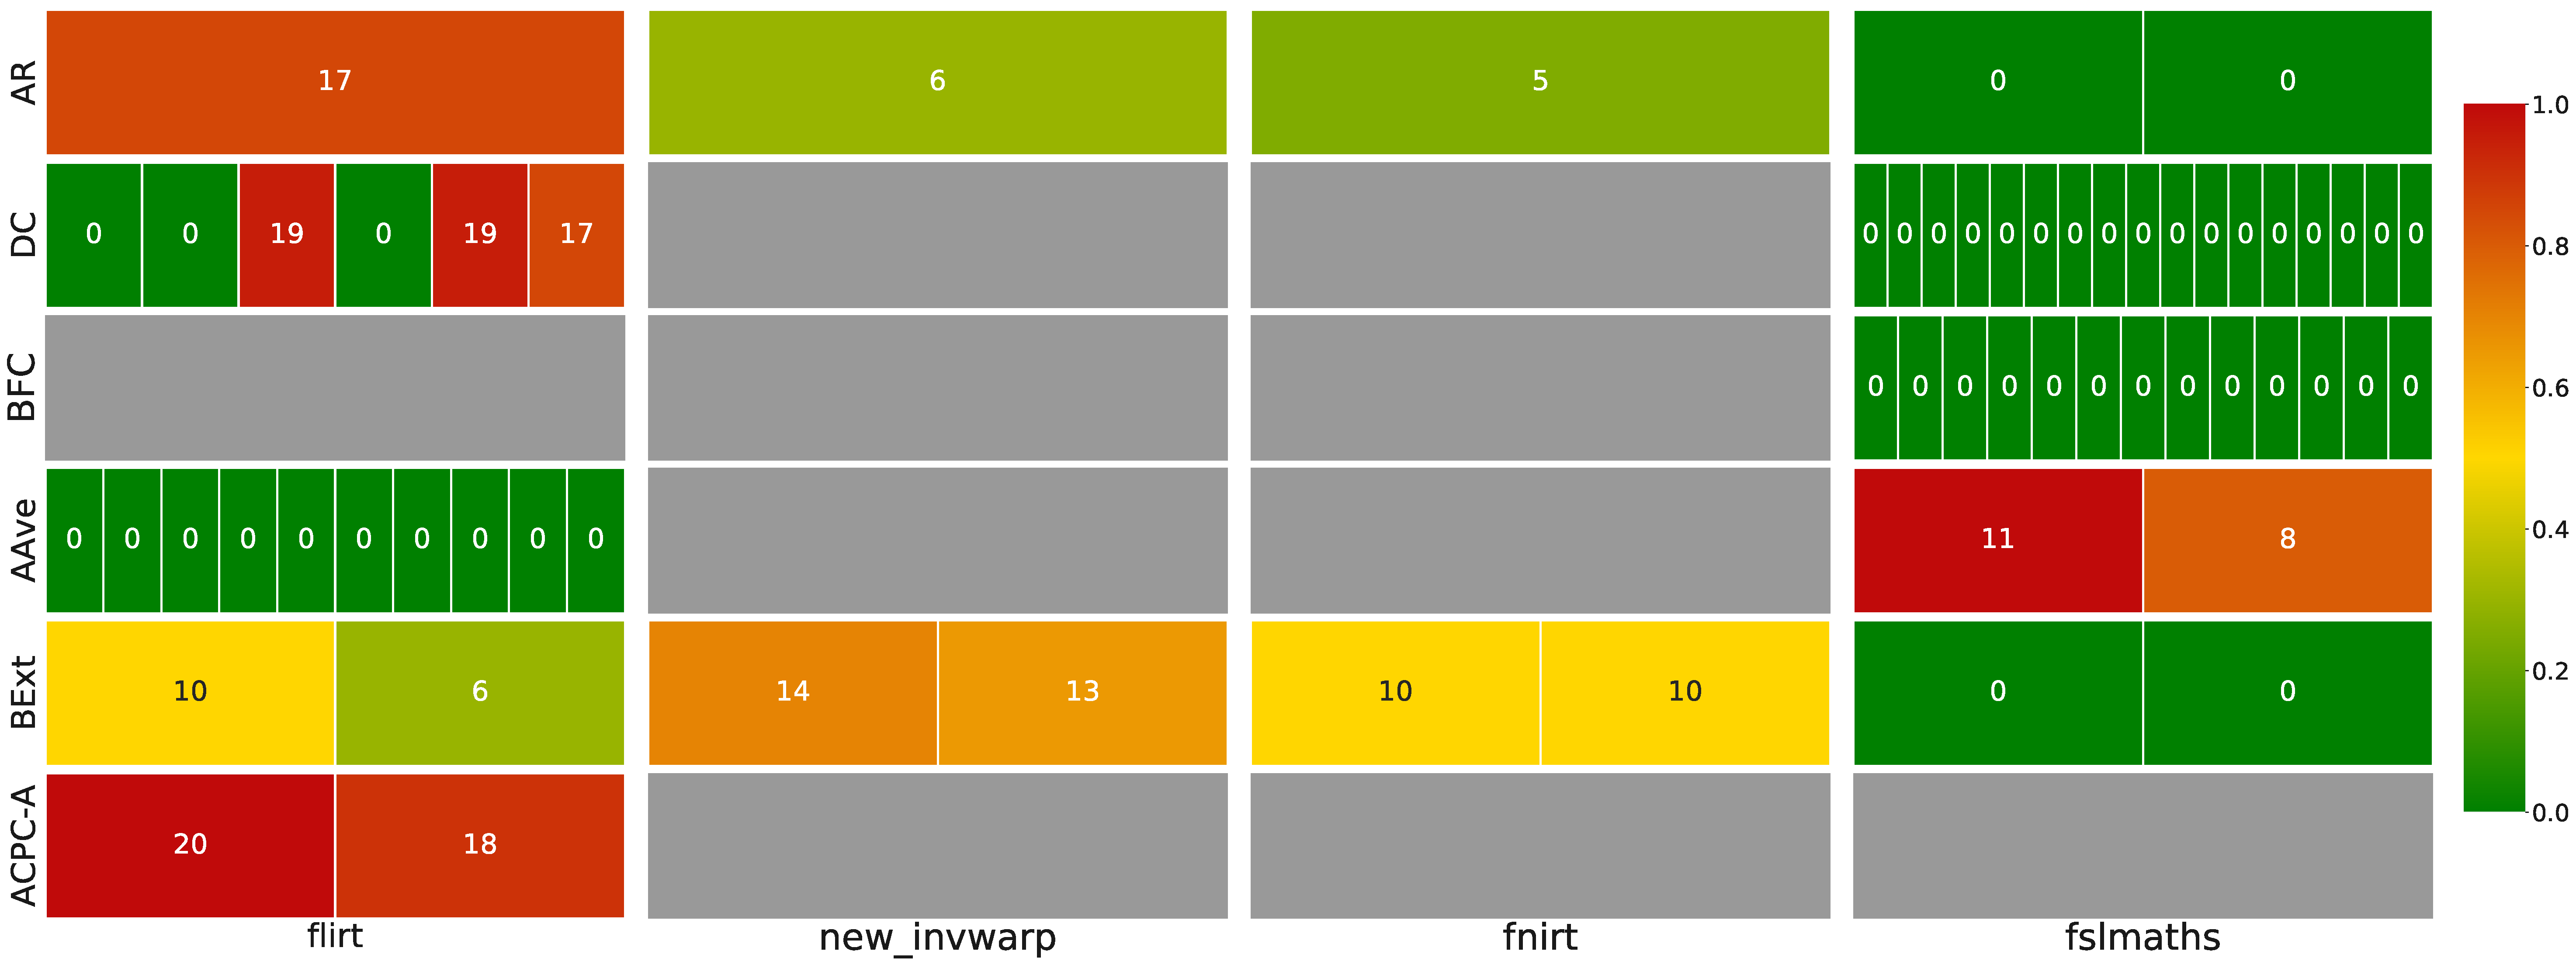
\includegraphics[width=\textwidth]{./figures/heatmap.pdf}
  \caption{Heatmap of non-reproducible processes across PreFreeSurfer pipeline steps.
  Each cell represents the occurrence of a particular command line in a
  pipeline step among Anatomical Average (AAve), Anterior/Posterior
  Commissure Alignment (ACPC-A), Brain Extraction (BExt), Bias Field
  Correction (BFC), or Atlas-Registration (AR). Cell labels indicate the
  fraction of subjects for which the corresponding process wasn't reproducible. For example,
  the \flirt tool was invoked 6 times in step DC for each of the 20
  subjects: 2 instances weren't reproducible in 19 subjects, 3
  instances were always reproducible, and 1 instance wasn't reproducible in
  17 subjects.
  \revised{Grey cells indicate that the process did not occur in the corresponding pipeline step.}}
  \label{fig:pfs_heatmap}
\end{figure*}

\begin{figure*}
   \centering
    \includegraphics[width=\linewidth]{figures/pfs-labeled.pdf}
    \caption{A complete provenance graph from the PreFreesurfer pipeline.
    \revised{Node labels use the same abbreviations as in Figure~\ref{fig:pfs_heatmap}.}
    For better visualization, processes associated with commands
    in \texttt{/bin} or \texttt{/usr/bin} were omitted, as well as
  \texttt{imtest}, \texttt{imcp}, \texttt{remove\_ext}, \texttt{fslval}, \texttt{avscale}, and \texttt{fslhd}.}
    \label{fig:complete_pfs}
\end{figure*}

\revised{
Figure~\ref{fig:fnirt_result} compares \fnirt results in Brain Extraction
for a particular subject using the checkerboard pattern,
a common method to illustrate the magnitude of the differences in registration results.
Differences appear to be visually important, in particular in the areas framed in red.}

\begin{figure}
  \centering
    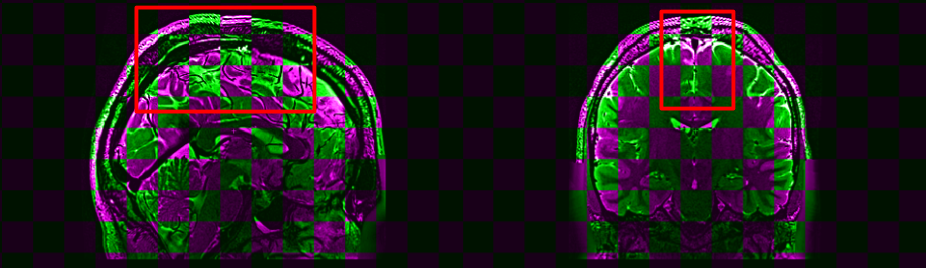
\includegraphics[width=\columnwidth]{figures/t2w_alignment.png}
    \caption{Differences between T2 \fnirt results in PreFreeSurfer's Brain Extraction (CentOS6 vs CentOS7).
    \revised{
    The colored squares indicate results obtained with CentOS6 (in purple) and CentOS7 (in green).
    The red boxes highlight regions with significant differences between the two OSes. }
    An animated version of the comparison is available \href{https://github.com/big-data-lab-team/HCP-reproducibility-paper/blob/master/figures/pfs_t2w_alignment.gif}{here} for better visualization.}
    \label{fig:fnirt_result}
\end{figure}

\subsubsection{Between-OS differences in FreeSurfer}

The only non-reproducible process identified by \toolname in FreeSurfer was
\texttt{mris\_make\_surfaces} (cortical and white matter surfaces
generation), a dynamically-linked executable
that produced different results for
10 out of 20 subjects.

However, FreeSurfer results still differ between conditions, due to the
propagation of differences created in PreFreeSurfer. We
observed the effect of this propagation in FreeSurfer results, as shown in
Figure~\ref{fig:tissue_class} for whole-brain segmentations. The
Dice coefficients associated with the 44 regions segmented by
FreeSurfer are shown in Figure~\ref{fig:scatter_plot}, showing that Dice coefficents below 0.9 are
observed in most regions, and particularly in the smallest ones.
\revised{However, no significant correlation between the Dice values and the region sizes was found
(Pearson's coefficient = 0.12, p-value = 0.43).}

\begin{figure}
%  \includegraphics{brain\_classification}
\centering
  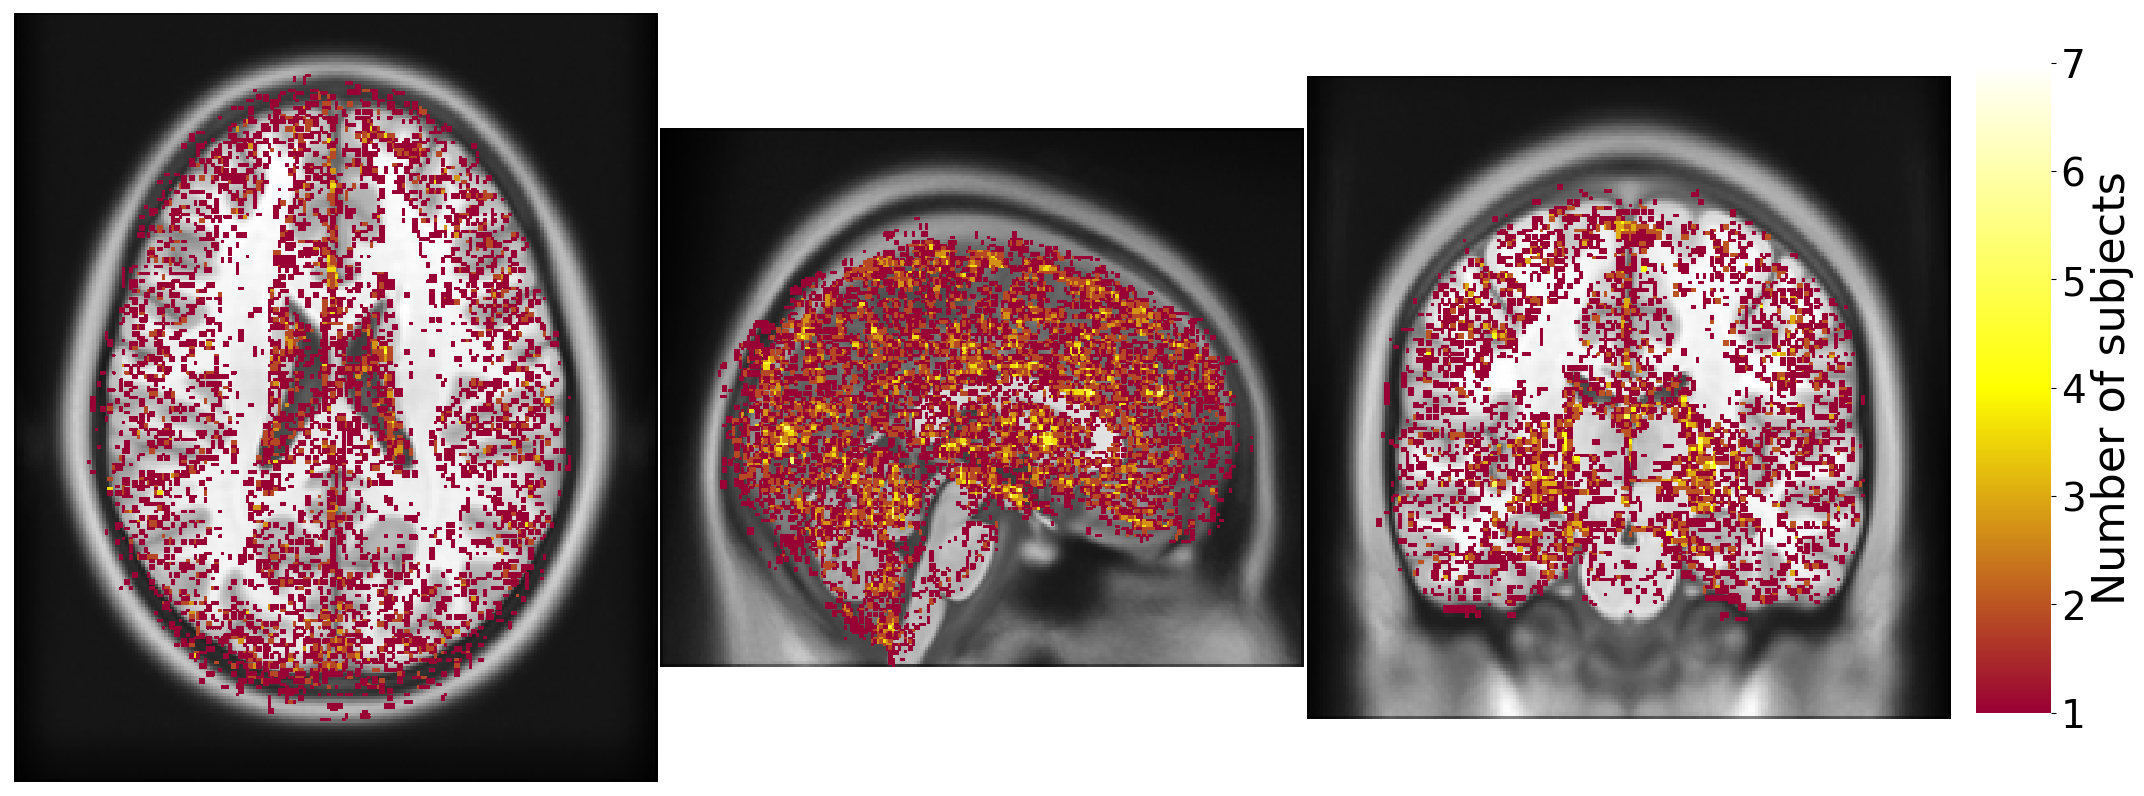
\includegraphics[width=\columnwidth]{figures/brain_segmentation_mni.png}
  \caption{Sum of binarized differences between whole-brain FreeSurfer
  segmentations obtained from PreFreeSurfer processings in CentOS6 vs CentOS7
   (N=20). Segmentations were resampled and overlaid to the MNI152 volume
  template.
  \revised{
  Each voxel shows the number of subjects for which different results were observed between CentOS 6 and CentOS 7.}
  An animated comparison of segmentations obtained for a particular subject is available
\href{https://github.com/big-data-lab-team/HCP-reproducibility-paper/blob/master/figures/fs_brain_segmentation.gif}
{here} for better visualization.}
  \label{fig:tissue_class}
\end{figure}

\begin{figure*}
  \hspace*{-1cm}
  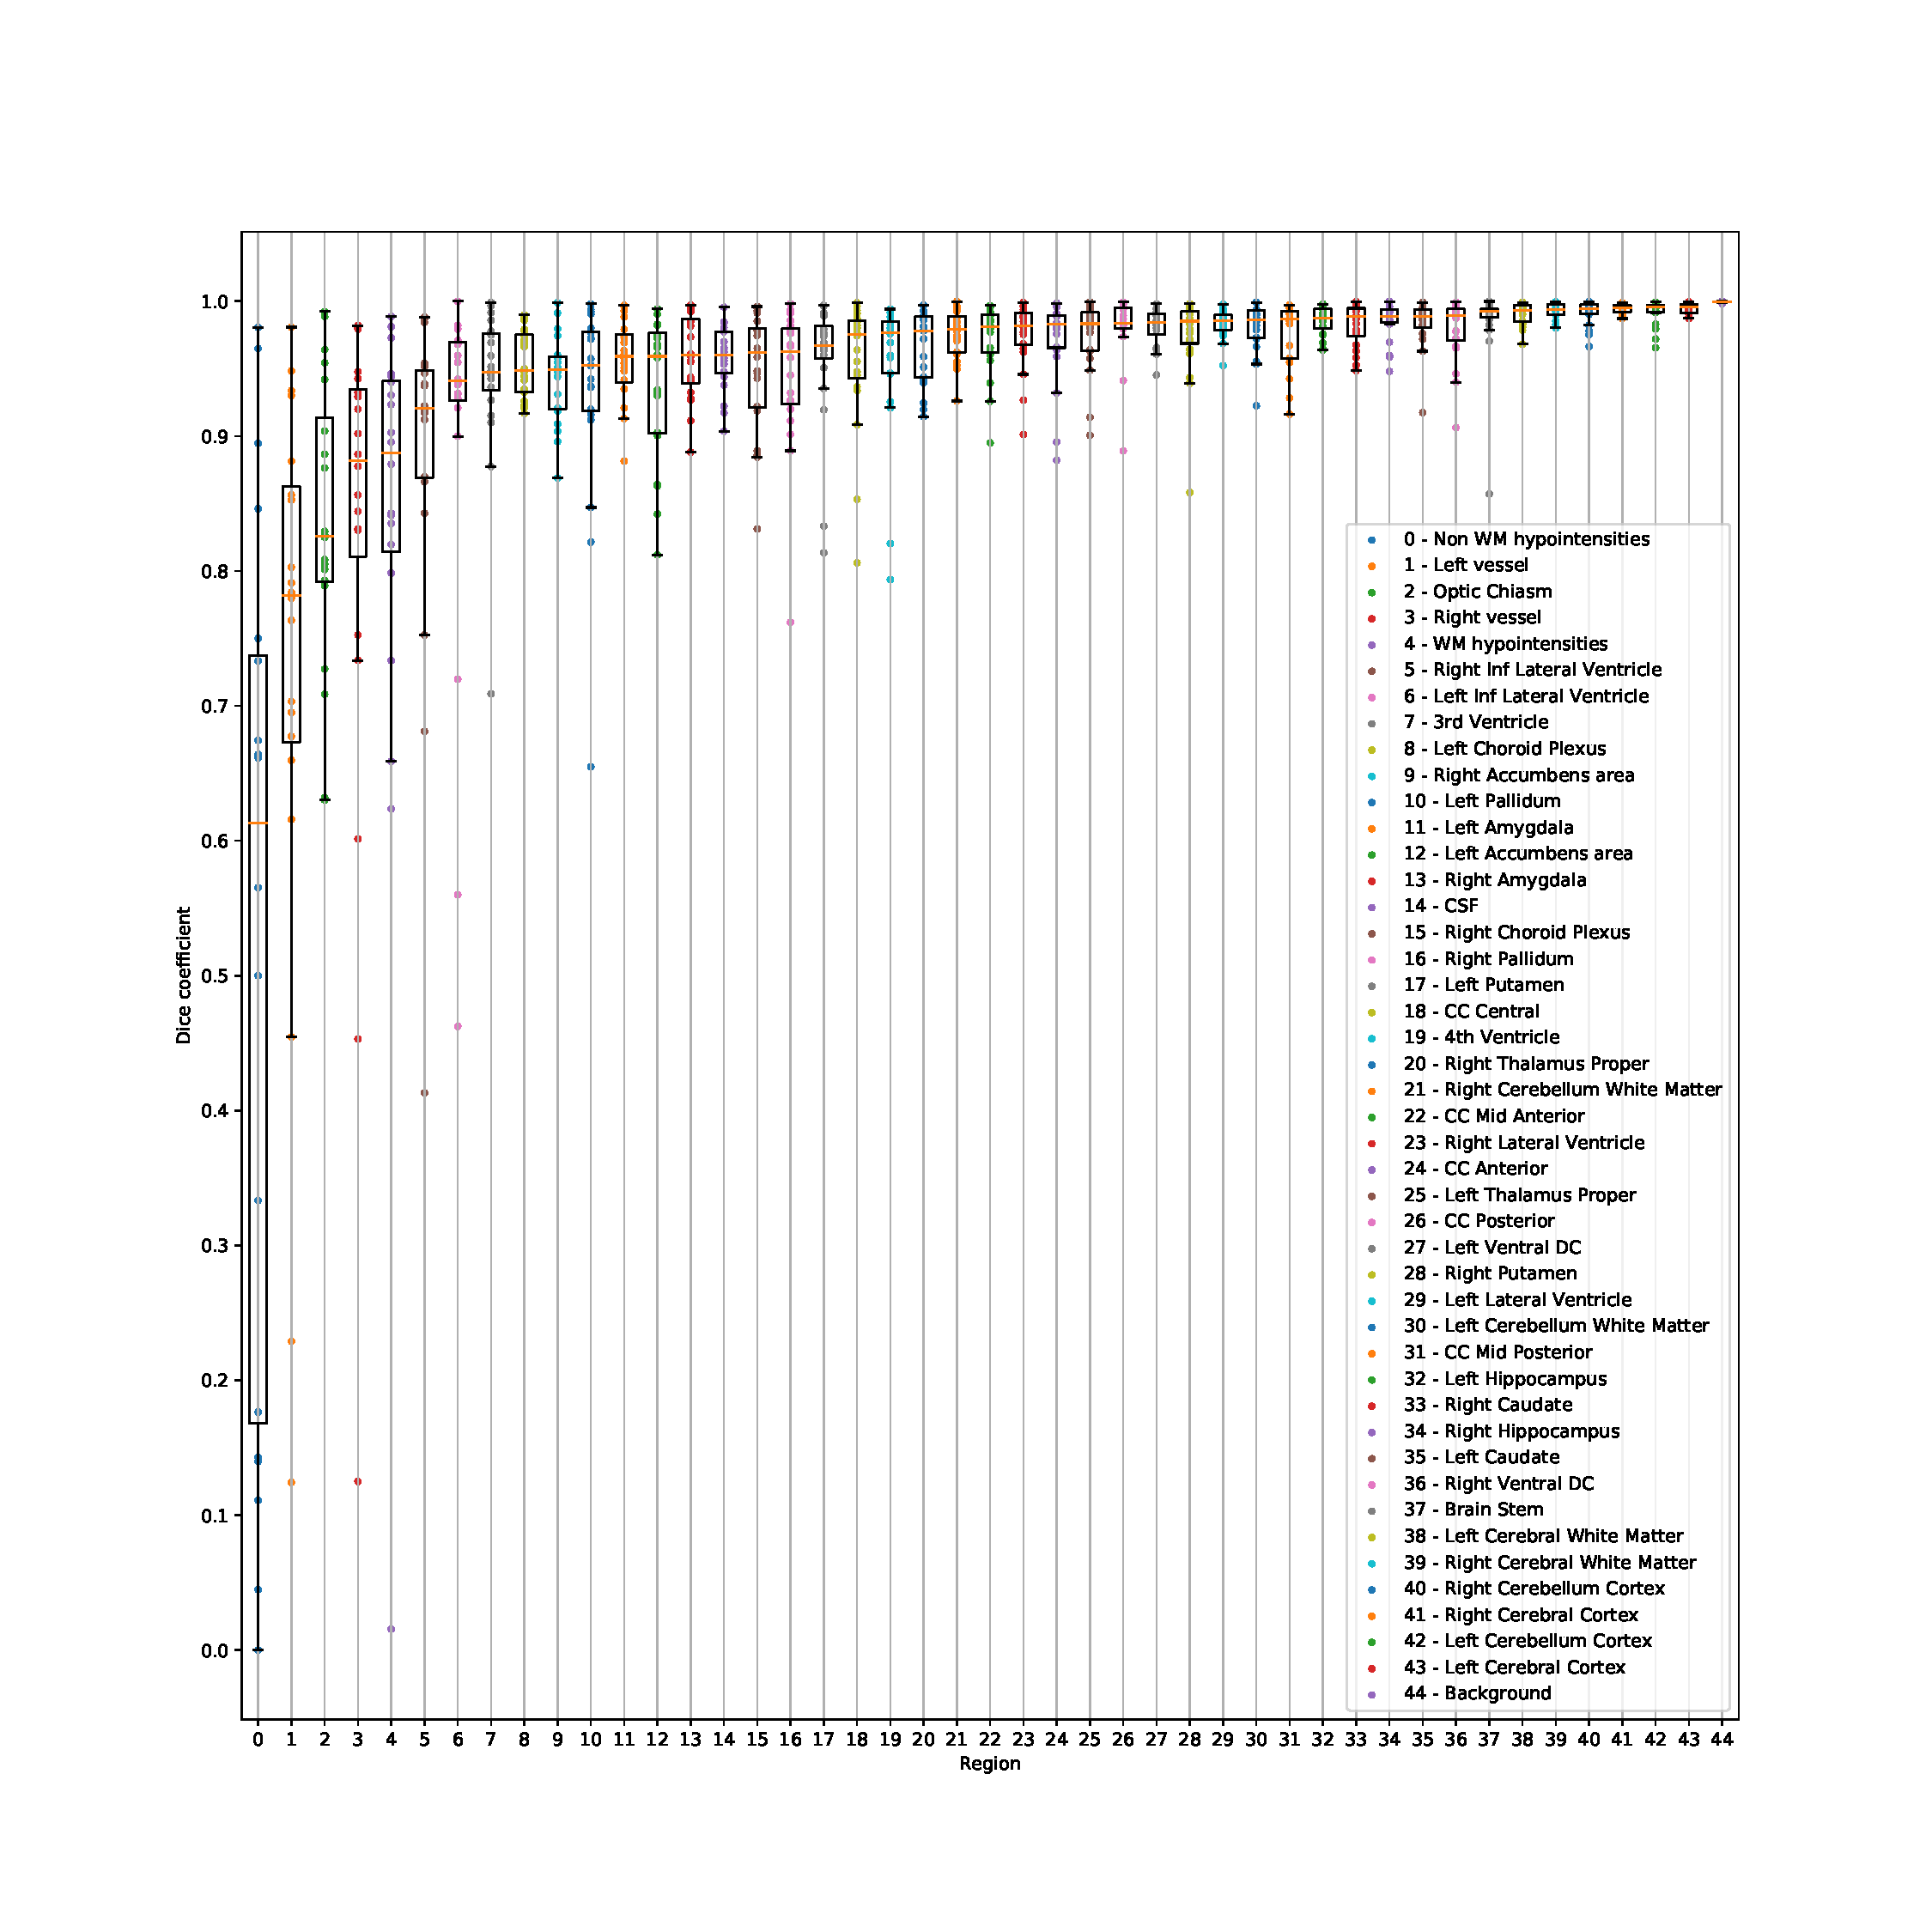
\includegraphics[width=1.1\linewidth]{figures/dice_regions.pdf}
    \caption{Dice coefficients between regions segmented by FreeSurfer in CentOS6 vs CentOS7 (N=20), ordered by increasing
    median values.
    \revised{Each point represents the Dice coefficient between segmentations of a particular region obtained in CentOS 6 vs CentOS 7 for a given subject.}
    Boxes brightness is proportional to the logarithm of the corresponding brain region size.}
    \label{fig:scatter_plot}
  \end{figure*}

  % We formulated the linear regression model for the Dice and region size variables as:
  % \[D=1 + T\epsilon ;    T=\frac{-1}{\overline{R}}\]
  % It is easier to obtain high overlaps with large regions,
  % while smaller regions are harder to be similarly segmented.
  % We obtained the epsilon value of $\approx$ 8.3 voxels ($\approx$ 3mm) which indicate the minimum number
  % of voxels in each region that needs to be segmented.


\section{Discussion}

Our results provide insights on the reproducibility of
neuroimaging pipelines, and on the relevance of the approach implemented
in \toolname for reproducibility studies.

\subsection{Key findings}
Linear and non-linear registration with FSL were found to
frequently lead to differences between results obtained with different
operating systems. This does not come as a surprise given the instabilities
associated with these processes. It also corroborates our previous findings
in~\cite{Glatard2015}, where fMRI pre-processing with FSL was found to vary across operating systems
starting from the motion
correction step, a step that uses FSL's \flirt tool internally. It
would be relevant to investigate if the observed instability of
registration processes generalizes to other toolkits, or if it remains specific
to FSL. In view of the effect of small data perturbations in a variety of
toolboxes and processes, such as cortical surface extraction using
FreeSurfer and CIVET~\cite{Lewis2017-ll} or connectome estimation using
Dipy~\cite{kiar2019comparing}, it is probable that this observation
generalizes widely across toolboxes and requires a deeper investigation of
the stability of linear and non-linear registration.

While only a handful or processes were found non-reproducible across the
tested operating systems, the effect of such instabilities were found to
propagate widely in the pipelines, and to substantially impact the segmentations
created by FreeSurfer. This illustrates the need to conduct reproducibility studies
on entire pipelines rather than isolated processes. It also highlights the need
for a deeper stability analysis of pipeline processes.

As is shown in Figure~\ref{fig:pfs_heatmap}, the reproducibility of
a given tool may vary across subjects and across processing parameters. For
instance, linear registration with \flirt seems to be fully reproducible in
the Anatomical Average sub-pipeline, while it is highly non-reproducible in
ACPC Alignment. In Brain Extraction, the same tool was found reproducible
for some subjects only. Therefore, reproducibility studies need to be
performed on several subjects. While this is common practice to some extent in neuroimaging,
software tests are often executed only on a single dataset to reduce the
associated computational load. Our results show that pipeline tests should
encompass enough subjects to cover execution paths adequately.

Our results illustrate the type of variability that can be introduced in
 neuroimaging results due to operating system updates. The
 numerical noise introduced by operating system updates is realistic, as
 such updates are likely to occur throughout the time span of a
 neuroscience study, but it is also uncontrolled, as it originates in
 updates of low-level libraries by third-party developers. A possible
 method to study this problem more comprehensively would be to introduce
 controlled numerical perturbations in pipelines, which could be done by
 introducing noise either in the data, or in floating-point computations
 through Monte-Carlo Arithmetic~\cite{Parker1997-qq}. The work
 in~\cite{kiar2019comparing} discusses and compares these two techniques.

\subsection{\toolname evaluation}

The processes identified by \toolname as non-reproducible were all
associated with dynamically-linked executables.
This makes complete sense as statically-linked executables are not
impacted by library updates. Moreover, the hypothetical effects of
hardware or Linux kernel updates were not measured, as the different
operating systems were deployed in Docker containers on the same host, that
is, using the same kernel and hardware.

\revised{
To evaluate the reproducibility of a pipeline, \toolname needs to execute it 5 times 
in order to (1) record a first \reprozip trace, (2) save transient files in the first condition, 
(3) compare results in the second condition, and repeat steps (2) and (3) for the other order of execution. 
It might be possible to further reduce this overhead by executing at step (2) only the processes 
depending on transient files, and capturing the transient files for the second condition simultaneously at step (3).}

We demonstrated the applicability of our approach by evaluating two of the
arguably most complex pipelines in neuroimaging. Technically, these
pipelines consist of a mix of tools assembled from different toolboxes
through a variety of scripts written in different languages. Our file-based
approach, notably enabled by \reprozip, was able to analyze these pipelines
without requiring their instrumentation, which saved a very substantial
technical effort. The assumptions made on the pipeline structure, related
to the absence of concurrent writes, were not violated in our analysis, and
are likely to not impede \toolname's applicability to the most common
neuroimaging pipelines.

\revised{
% Furthermore, we can use methods to ensure that enough tests have been performed for labeling a tool as reproducible.
% We approved the irreproducibility of the tools, but we cannot say a tool is reproducible since
\toolname labels pipeline processes based on the tested dataset, 
while the reproducibility of the tools can be changed over the new datasets. 
In this regard, we need to confirm the reproducibility of the tools over all the possible 
subject diversity and processing parameters. 
We can rely on the code coverage to measure the proportion of the code covered by the tests. 
Ideally, the code coverage as close to 100\% as possible ensures that most of the code is fully tested. 
This is a key principle of reproducibility to guarantee the appropriate testing of the tools. 
Having sufficient subject tests so that covers most of the code could increase confidence to confirm 
the reproducibility of the tools.
As another solution, we can estimate the probability of the tool reproducibility based on 
the number of subjects that the tool was tested as reproducible. To this order, 
we refer to the probability measurement used in~\cite{glatard2015classifications}, which can state that the probability 
to observe all reproducible results among $N’$ future tests given that $n$ non-reproducible results happened among $N$ 
previous tests is:

\[p(N',n,N)=\frac{N+1}{N+N'+1}\frac{\binom Nn}{\binom {N+N'}n}\]

This formula gives a high probability to see reproducible results from the tools have been tested on a high series of 
subjects as reproducible.
}

File-based analyses also have limitations related to the
granularity at which they operate. Indeed, differences can only be
identified at the level of an entire operating-system process, which can
correspond to arbitrary amounts of code. Narrowing down the analysis to
particular libraries, functions, or even code sections would require
another approach. Similarly, \toolname would not be able to detect
differences in data not saved in files but instead passed to subsequent processes
in memory. A common scenario in neuroimaging pipelines is that tools return
results in their standard output, which is parsed by the calling process
and passed to subsequent ones through variables.

\revised{
Computational environments are only one of many factors contributing to the
on-going reproducibility crisis. In fact, sample size selection,
publication bias, or methodological flexibility in the analysis are likely
to have a stronger effect than numerical perturbations, although
to our knowledge no evidence of this is available. We refer to the
studies in~\cite{botvinik2020variability,bowring2019exploring,bhagwat2020understanding,kennedy2019everything} for deeper
analyses of the associated effects on neuroimaging analyses. It should also be
noted that the effects of computational environments and these other
factors manifest at different levels: referring to the terminology used
in~\cite{peng2011reproducible}, computational environments are associated with
\emph{reproducibility}, the minimal standard by which identical results
should be obtainable from identical data and parameters, while the other
aforementioned factors belong to \emph{replicability}, the ultimate
standard by which independent experimenters should be able to draw similar
conclusions from similar experiments. In practice, variability resulting
from computational environments manifests during software testing (test
results depend on execution platform), deployment on HPC systems (results
obtained on local vs HPC systems differ), or software version updates
(results obtained before vs after the update differ), while factors related
to replicability impact the community more broadly. Ultimately, both
reproducibility and replicability should be understood and improved.
}

\section{Conclusion}

We presented \toolname, a tool to detect the source of numerical
differences in complex pipelines executed in different computational
conditions. \toolname leverages system-call interception through the
\reprozip tool, and therefore can be applied to the most complex pipelines
without requiring their instrumentation. It is available at
\url{https://github.com/big-data-lab-team/spot} under MIT license.
% Moreover, we registered the spot tool in the bio.tools with the identifier biotools:spottool,
% and in the SciCrunch.org database with RRID (Research Resource Identifier) SCR\_018915.

By applying \toolname to the pre-processing pipelines of the Human
Connectome Project, compared in different operating systems, we showed that
between-OS differences are mostly originating in linear and non-linear
image registration tools. Moreover, differences introduced during image
registration propagate widely in the pipelines, leading to important
variability in whole-brain segmentations.

Future work will investigate in more details the numerical stability of
registration algorithms. Additionally, we plan on using Monte-Carlo arithmetic
to inject controlled amounts of noise in pipelines and monitor
uncertainty propagation and amplification in their results.

\revised{
\section{Availability of Source Code and Requirements}
\begin{itemize}
  \item Project name: \toolname
  \item Project home page:\url{https://github.com/big-data-lab-team/spot}
  \item Operating system: Linux
  \item Programming language: Python
  \item Other requirements: Python 3.6 or higher, \reprozip, Docker, and Boutiques
  \item License: MIT License
  \item Biotools identifier: \href{https://bio.tools/spottool}{spottool}
  \item SciCrunch ID: RRID:SCR\_018915

\end{itemize}

\section{Supplementary Data}
Supplementary materials include Supplementary Table S1. Summary of the subjects used in the experiments.
}

\section{Acknowledgments}

We warmly thank Compute Canada (\url{http://www.computecanada.ca}) and Calcul
Qu\'ebec (\url{http://www.calculquebec.ca}) for providing the infrastructure used in our experiments.
Data and pipelines were provided by the Human Connectome Project, WU-Minn
Consortium (Principal Investigators: David Van Essen and Kamil Ugurbil;
1U54MH091657) funded by the 16 NIH Institutes and Centers that support
the NIH Blueprint for Neuroscience Research; and by the McDonnell
Center for Systems Neuroscience at Washington University.
%\tristan{check ethics}


\bibliographystyle{plain}
\bibliography{biblio}

\end{document}
